\documentclass[12pt,a4]{article}




\usepackage{graphicx,amsmath,amssymb,amsthm, boxedminipage,xcolor,amscd,amsbsy,latexsym,url,bm}

%\usepackage[lined,boxed]{algorithm2e}

\usepackage{algorithm}
\usepackage{algpseudocode}


\newtheorem{theorem}{Theorem}[section]
\newtheorem{proposition}[theorem]{Proposition}
\newtheorem{lemma}[theorem]{Lemma}
\newtheorem{corollary}[theorem]{Corollary}
\newtheorem{definition}[theorem]{Definition}

\newtheorem*{theorem*}{Theorem}
\newtheorem*{lemma*}{Lemma}
\newtheorem*{solution}{Solution}
\newtheorem*{proposition*}{Proposition}


\newtheorem{exercise}[theorem]{Exercise}
\newtheorem{exerciseD}[theorem]{*Exercise}
\newtheorem{exerciseDD}[theorem]{**Exercise}

\let\oldexercise\exercise
\renewcommand{\exercise}{\oldexercise\normalfont}

\let\oldexerciseD\exerciseD
\renewcommand{\exerciseD}{\oldexerciseD\normalfont}

%\let\oldexerciseD\exerciseD
%\renewcommand{\exerciseD}{\oldexerciseD\normalfont}

%\let\oldexerciseDD\exerciseDD
%\renewcommand{\exerciseDD}{\oldexerciseDD\normalfont}

\newcommand{\E}{\mathbb{E}}
%\newcommand{\nth}[1]{#1^{\textsuperscript{th}}}
\newcommand{\scalar}[2]{\ensuremath{\langle #1, #2\rangle}}
\newcommand{\floor}[1]{\left\lfloor #1 \right\rfloor}
\newcommand{\ceil}[1]{\left\lceil #1 \right\rceil}
\newcommand{\norm}[1]{\|#1\|}
\newcommand{\pfrac}[2]{\left(\frac{#1}{#2}\right)}
\newcommand{\nth}[1]{#1^{\textsuperscript{th}}}
\newcommand{\core}{\textnormal{core}}



\newif\ifsolution

\solutionfalse

\newcommand{\answer}[1]{
\ifsolution
{\color{blue} #1}
\else
\fi
}



\newcommand{\poly}{\textnormal{poly}}
\newcommand{\quasipol}{\textnormal{quasipol}}
\newcommand{\ssubexp}{\textnormal{stronglySubExp}}
\newcommand{\wsubexp}{\textnormal{weaklySubExp}}
\newcommand{\simplyexp}{\textnormal{E}}
\newcommand{\expo}{\textnormal{Exp}}



\newcommand{\N}{\mathbb{N}}
\newcommand{\nn}{\mathbb{N}_0^n}
\newcommand{\R}{\mathbb{R}}
\newcommand{\Z}{\mathbb{Z}}


\definecolor{darkgreen}{rgb}{0,0.6,0}

\date{}

\title{
\hbox{  Mathematical Foundations of Computer Science}
  \vspace{3mm}
{\normalsize CS 499,	Shanghai Jiaotong University,  Dominik Scheder\\
%\vspace{3mm}
Spring 2019}
}


\begin{document}

\maketitle

%\begin{quotation}
%  You are welcome to discuss the exercises in the discussion
%  forum. Please take them serious. Doing the exercises is as important
%  than watching the videos.
%
%  I intentionally included very challenging exercises and marked them
%  with one or two ``$*$''. No star means you should be able to solve
%  the exercises without big problems once you have understood
%  the material from the video lecture. One star means it requires 
%  significant additional thinking. Two stars means it is not 
%  unlikely that you will fail to solve them, even once you have understood
%  the material and thought a lot about the exercise. Don't feel bad
%  if you fail. Failure is part of learning.
%
%  This is the first time this course is online. Thus there might be mistakes
%  (typos or more serious conceptual mistakes) in the exercises. I will be 
%  grateful if you point them out to me!
%\end{quotation}

\begin{document}



\setcounter{section}{4}
\begin{center}
  \large\textbf{Group: navigator} 
\end{center}
\begin{center}
  \begin{tabular}{rl}
 Xu Huan  & 517021910724 \\
 Tianyao Shi     &     517021910623 \\
Chenxiao Yang    &    517021910540  \\
Jiaqi  Zeng      &     517021910882  \\
  \end{tabular}
\end{center}

\newpage
\section{The Graph Score Theorem}



\begin{itemize}
 \item Homework assignment published on Thursday, 2019-03-27.
 \item Submit questions and first solution by Wednesday, 2019-04-03, by
 email to dominik.scheder@gmail.com and the TAs.
 \item You will receive feedback by Monday, 2019-04-08.
 \item Submit your final solution by Sunday, 2019-04-14 to me and the two TAs.
\end{itemize}



\begin{exercise}
  Describe, in simple sentences with a minimum of mathematical formalism, (1) the score
  of a graph, (2) what the graph score theorem is, (3) the idea of the
  graph score algorithm, (4) where the difficult part of its proof is.
  Imagine you have a friend who does not take this class, and think about how to answer
  the above questions to them.
\end{exercise}
\begin{proof}
  \begin{enumerate}
    \item
    Assume that we have a graph $G=(V,E)$. Define $d_i$ be the degree of the i$^th$ vertex. Then $score(G)=(d_1,d_2,\cdots,d_n)$.
    \item
    \textbf{Theorem}

    Let $\textbf{d}=(d_1,d_2,\cdots,d_n)$ with $d_1 \leq \cdots \leq d_n$. Define $\textbf{d'}$ by
    \begin{equation*}
    d':=
    \begin{cases}
    \ d_i-1 & \text{for } i=n-d_n,\cdots,n-1 \\
    \ d_i & \text{for } i=1,\cdots,n-d_n-1 \\
    \end{cases}
    \end{equation*}


  Then there exists a graph with score \textbf{d} if and only if there exists a graph with score \textbf{d'}.

  \item
  \textbf{Graph Score Algorithm:}

  find-graph$(d_1,d_2,\cdots,d_n)$

  \quad  sort$(d_1,d_2,\cdots,d_n)$
    \begin{equation*}
    d':=
    \begin{cases}
    \ d_i-1 & \text{for } i=n-d_n,\cdots,n-1 \\
    \ d_i & \text{for } i=1,\cdots,n-d_n-1 \\
    \end{cases}
    \end{equation*}
  \quad \quad G':=find-graph$(d_1',d_2',\cdots,d_{n-1}')$

  \quad  if G'=null return null

  \quad  else G:=
    \begin{figure}[htbp]
        \centering
        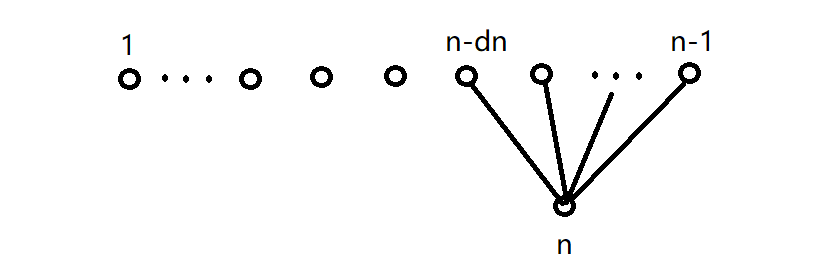
\includegraphics[width=0.5\textwidth]{1.jpg}
    \end{figure}

    \item
    To prove the above theorem, we see that we can easily find a graph with \textbf{d} from \textbf{d'}. That is to create a point $n$ and connect it to all points from $n-d_n$ to $n-1$. But it is not equally easy to prove the other side.
  \end{enumerate}
\end{proof}


\subsection{Alternative Graphs}

Now we will look at different notions of graphs. As defined in class and in the video
lectures, a graph is a pair $G = (V,E)$ where $V$ is a (usually finite) set, called the {\em vertices},
and $E \subseteq {V \choose 2}$, called the set of {\em edges}.

\paragraph{Multigraphs.}
A {\em multigraph} is like a graph, but you can have several parallel edges between
two vertices. You cannot, however, have self-loops. That is, there cannot
be an edge from $u$ to $u$ itself. This is an example of a multigraph:

\begin{center}
  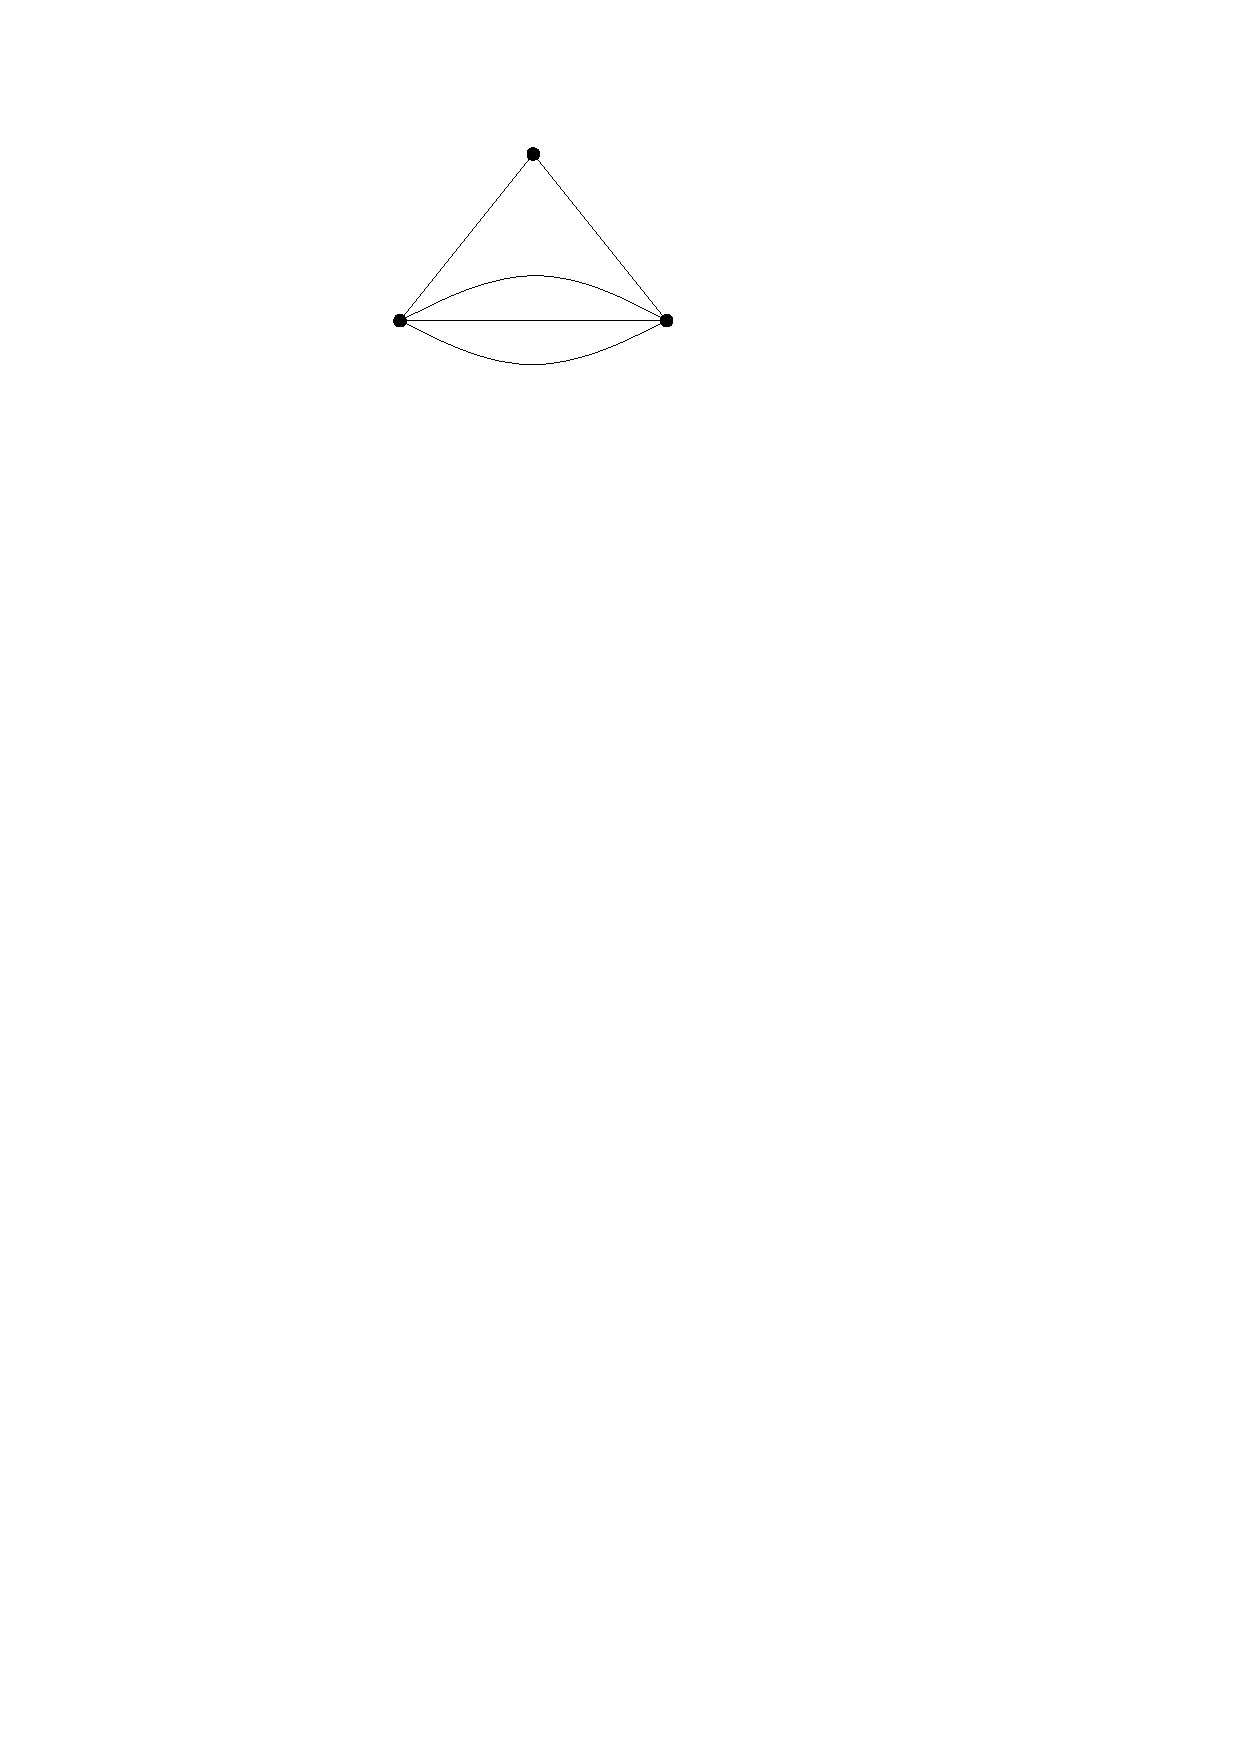
\includegraphics[width=0.25\textwidth]{figures/multigraph-score.pdf}
\end{center}

We can define degree and score for multigraphs, too. For example, this multigraph
has score $(4,4,2)$. Obviously no graph
can have this score.



\begin{exercise}
  State a score theorem for multigraphs. That is, something like
  \begin{theorem}[Multigraph Score Theorem]
     Let $(a_1,\dots,a_n) \in \N_0^n$. There is a multigraph
     with this score if and only if \texttt{\textup{<fill in some simple criterion here>}}.
  \end{theorem}


  \textbf{Remark.} This is actually
  simpler than for graphs.
\end{exercise}

\begin{exercise}
  Prove your theorem.
\end{exercise}

\begin{proof}

  \textbf{Theorem}

  Let $\textbf{d}=(d_1,d_2,\cdots,d_n)$ with $d_1 \leq \cdots \leq d_n$. Define $\textbf{d'}$ by
  \begin{equation*}
  d':=
  \begin{cases}
    \
  \begin{cases}
  \ d_i-1 & \text{for } i=n-d_n,\cdots,n-1 \\
  \ d_i & \text{for } i=1,\cdots,n-d_n-1 \\
  \end{cases}
  \text{if } n \geq d_n \\
  \\
  \
  \begin{cases}
  \ d_i-1 & \text{for } i=1,\cdots,n-1 \\
  \ d_i-(n-1) & \text{for } i=n \\
  \end{cases}
  \text{if } n<d_n
\end{cases}
  \end{equation*}

Then there exists a graph with score \textbf{d} if and only if there exists a graph with score \textbf{d'}.
\\
\\
\textbf{Proof:}

\textbf{If $n \geq d_n$:}

d' $\Rightarrow$ d:
It is easy to find d based on d'. We just need to create a point $n$ and connect it to all points from $n-d_n$ to $n-1$.

d $\Rightarrow$ d':

\textbf{Claim1}:
If $\exists$ G such that $score(G)=(d_1,d_2,\cdots,d_n)$, then $\exists$ G such that $score(G)=(d_1,d_2,\cdots,d_n)$ and in which exists a point $n$ that connects to all points from $n-d_n$ to $n-1$.

With this claim, $G-n=:G'$, $score(G')=d'$.

Now we prove the claim. Define j(G) be the largest number j such that vertex n has an edge to vertex $n-1,n-2,\cdots,n-j$.

\textbf{Claim2:}
If G maximizes j(G) then $j(G)=d_n$.

proof: Suppose not, then $j(G)<d_n$.
\begin{figure}[!htb]
    \centering
    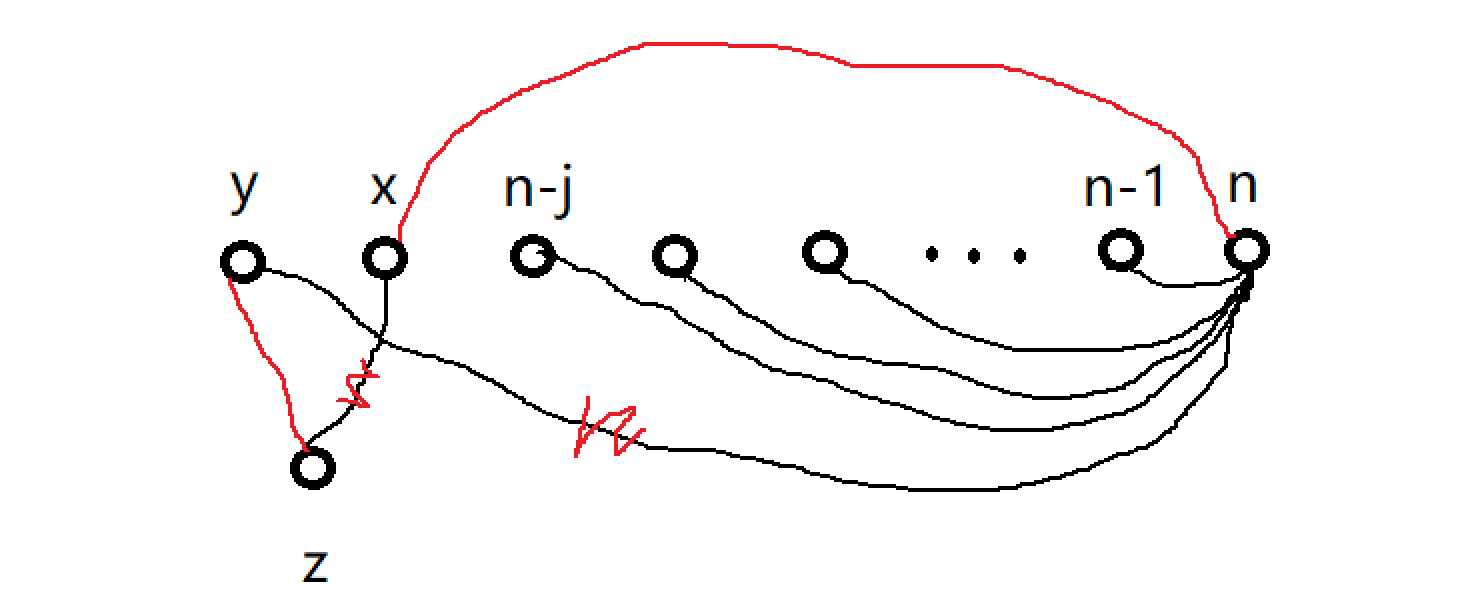
\includegraphics[width=0.5\textwidth]{2.jpg}
\end{figure}

As the figure above (the black lines), we obtain that: $\{ x,n\} \notin \E$, $deg(n)=d_n$, $\{ n,y\} \in \E$, $deg(y) \leq deg(x)$. Hence, $\exists$ vertex z such that $\{ x,z\} \in \E$ and $\{ y,z\} \notin \E$. We can replace $\{ n,y \}$ and $\{ x,z \}$ by $\{ n,x\}$ and$\{ y,z \}$.

Now we get a new graph H and we have $score(G)=score(H)$ but $j(H)>j(G)$. This contradicts with G maximizes j(G). So we have proved \textbf{Claim2} which can easily lead to \textbf{Claim1} and we finally prove $d \Rightarrow d'$.

\textbf{If $n < d_n$:}

d' $\Rightarrow$ d: It is also easy to find d based on d'. We just need to connect vertex n with all other vertices.

d $\Rightarrow$ d':

\textbf{Claim3}:
If $\exists$ G such that $score(G)=(d_1,d_2,\cdots,d_n)$, then $\exists$ G such that $score(G)=(d_1,d_2,\cdots,d_n)$ and in which exists a vertex $n$ that connects to all vertices from $1$ to $n-1$.

With this claim,
\begin{equation*}
G':= G- \sum_{k=1}^{n-1} \{k,n\}
\end{equation*}
and we have $score(G')=d'$.

Now we prove the claim. Define j(G) be the largest number j such that vertex n has an edge to vertex $n-1,n-2,\cdots,n-j$.

\textbf{Claim4:}
If G maximizes j(G) then $j(G)=n-1$.

proof: Suppose not, then $j(G)<n-1$.
\begin{figure}[!htb]
    \centering
    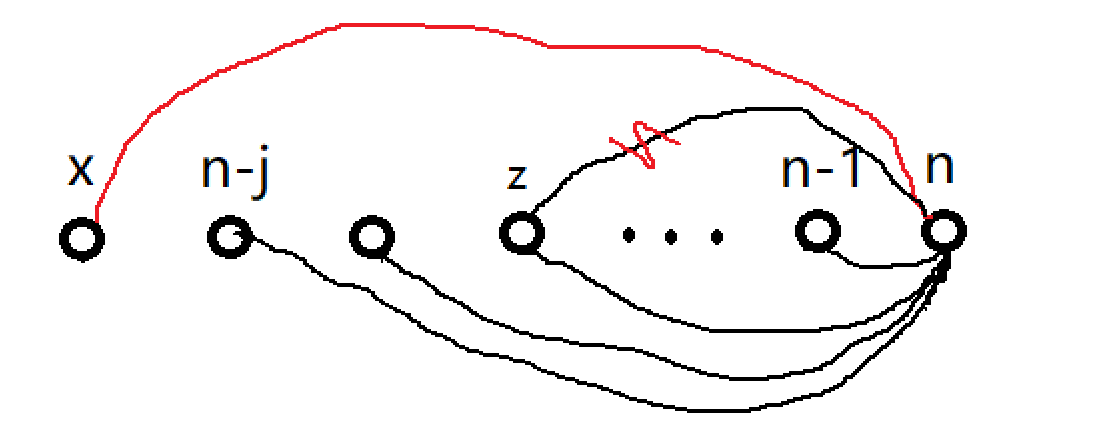
\includegraphics[width=0.5\textwidth]{3.jpg}
\end{figure}

As the figure above (the black lines), we obtain that: $x<j $ so $\{ x,n\} \notin \E$. Since $d_n>n$, there must exist an vertex z such that 2 edges are between vertex z and vertex n. We can replace one of them by an edge between vertex n and vertex x. Hence, we obtain a new graph H with a bigger j(H). Continue the operation, we may finally connect all other vertices with vertex n. This means $j(G)=n-1$ and leads to an contradiction.

Now we have proved \textbf{Claim4} and we can easily obtain \textbf{Claim3} and finally prove d $\Rightarrow$ d'.





\end{proof}

\newcommand{\wdeg}{\textnormal{wdeg}}

\paragraph{Weighted graphs.} A weighted graph is a graph in which every edge $e$ has a non-negative weight $w_e$.
In such a graph the {\em weighted degree} of a vertex $u$ is $\wdeg(u) = \sum_{ \{u,v\} \in E} w_{\{u,v\}}$.

\begin{center}
  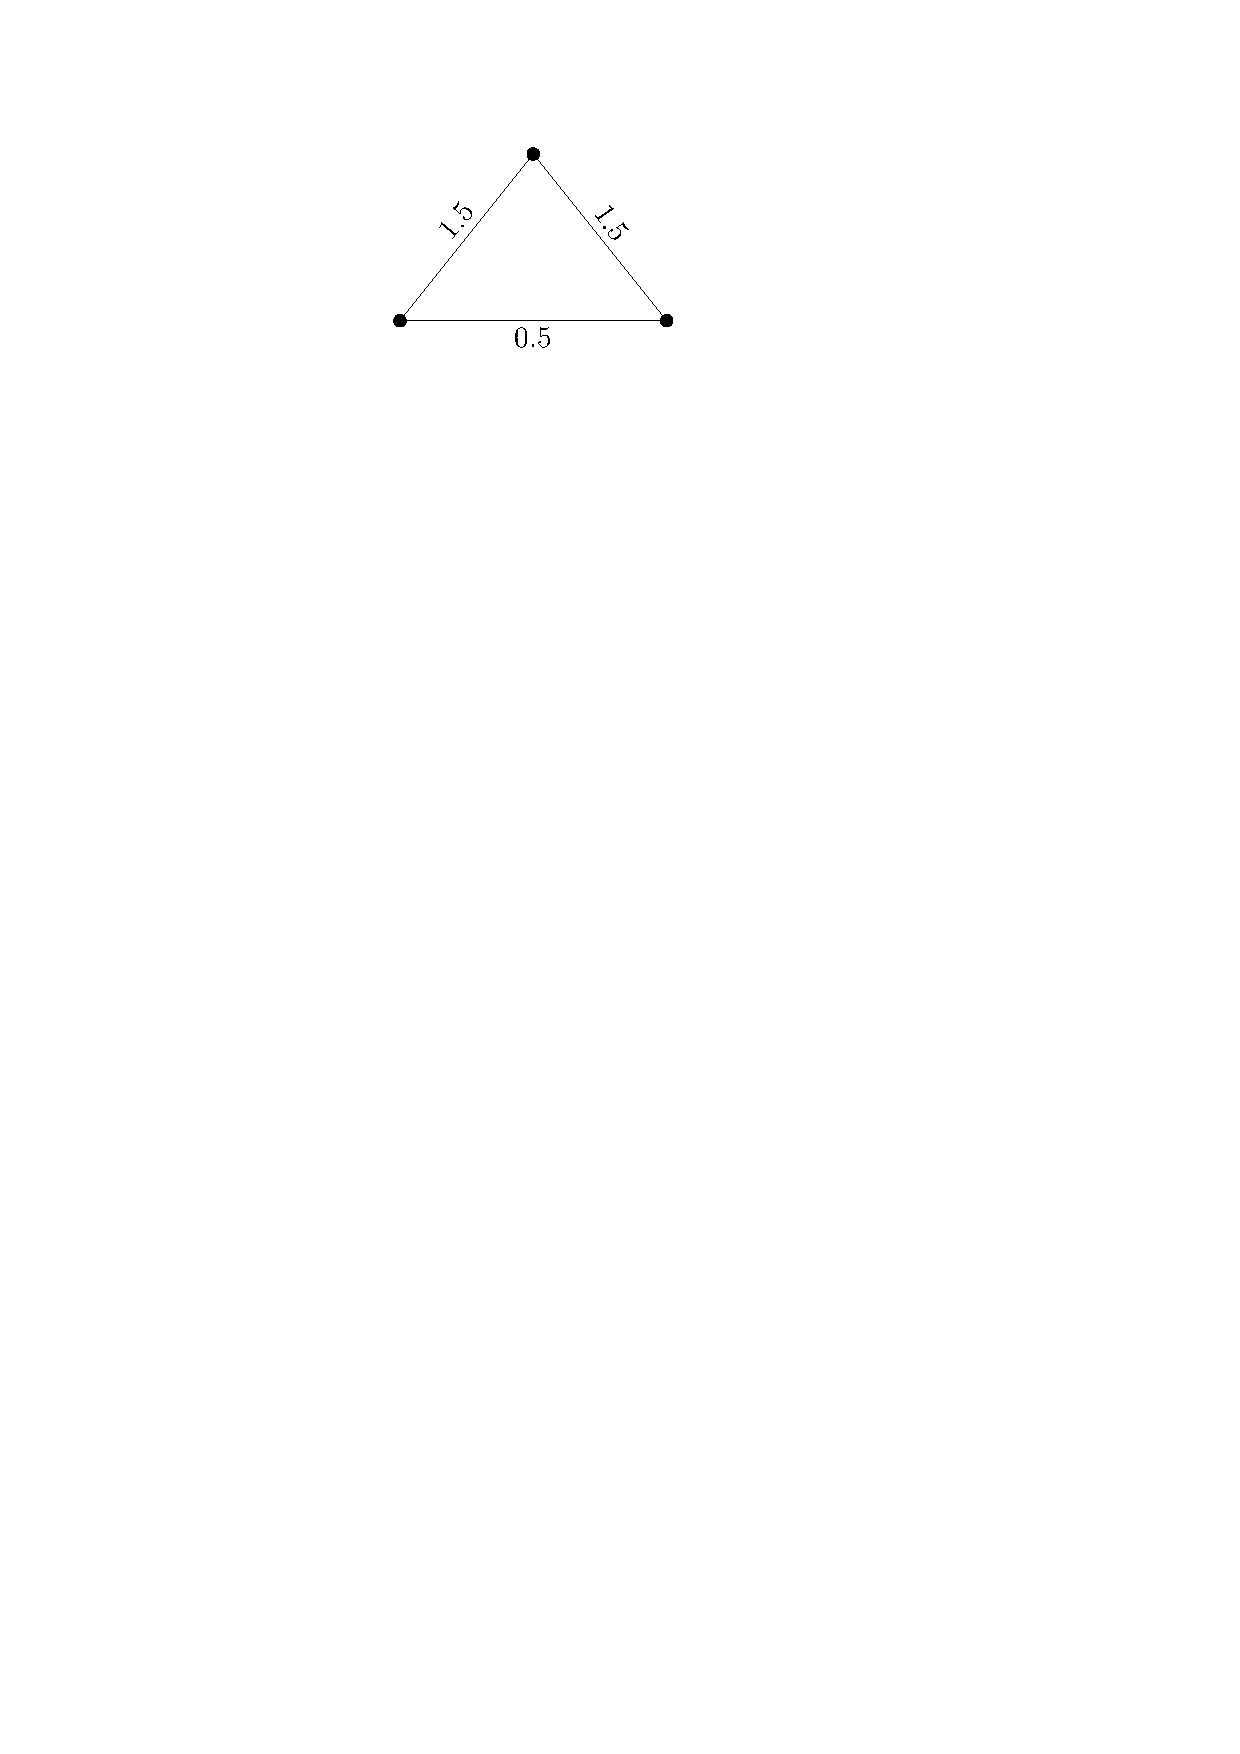
\includegraphics[width=0.25\textwidth]{figures/weighted-graph-score.pdf}
\end{center}

This is an example of a weighted graph, which has score $(3,2,2)$. Obviously no graph
and no multigraph can have this score.

\begin{exercise}
  State a score theorem for weighted graphs. That is, state something like
  \begin{theorem}[Weighted Graph Score Theorem]
     Let $(a_1,\dots,a_n) \in \R_0^n$. There is a weighted graph
     with this score if and only if \texttt{\textup{<fill in some simple criterion here>}}.
  \end{theorem}
  \textbf{Remark.} This
  is actually even simpler.
\end{exercise}


\begin{exercise}
  Prove your theorem.
  \begin{proof}
  \textbf{Theorem}
  Let $\textbf{d}=(d_1,d_2,\cdots,d_n)$ with $d_1 \leq \cdots \leq d_n$. Define $\textbf{d'}$ by
  $$
  d'= d_i-x_i ,\ \text{for } i=1,2,\cdots,n-1; \ 
  \sum\limits_{i = 1}^{n-1}x_i = d_n,\ x_i \in \mathbb{R}^+
  $$

Then there exists a graph with score \textbf{d} if and only if there exists a graph with score \textbf{d'}.
\\
\\
\textbf{Proof.}
\item $\rightarrow$: \par
If there exists a graph with score \textbf{d}, then the vertice whose degree is $d_n$ must have some edges with weight of $x_i$ connected to other vertices. Delete this vertice and related edges, the remains is obviously a graph with score \textbf{d'}.
\item $\leftarrow$:	\par
If there exists a graph with score \textbf{d'},  we can add vertice with degree of $d_n$ by creating several edges connected to vertices $\{v_1, v_2, \cdots, v_{n-1}\}$ whose weight is $x_i$. Then we get a weighted graph with score \textbf{d}.
  \end{proof}
\end{exercise}

\paragraph{Allowing negative edge weights.} Suppose now we allow negative edge weights, like here:
\begin{center}
  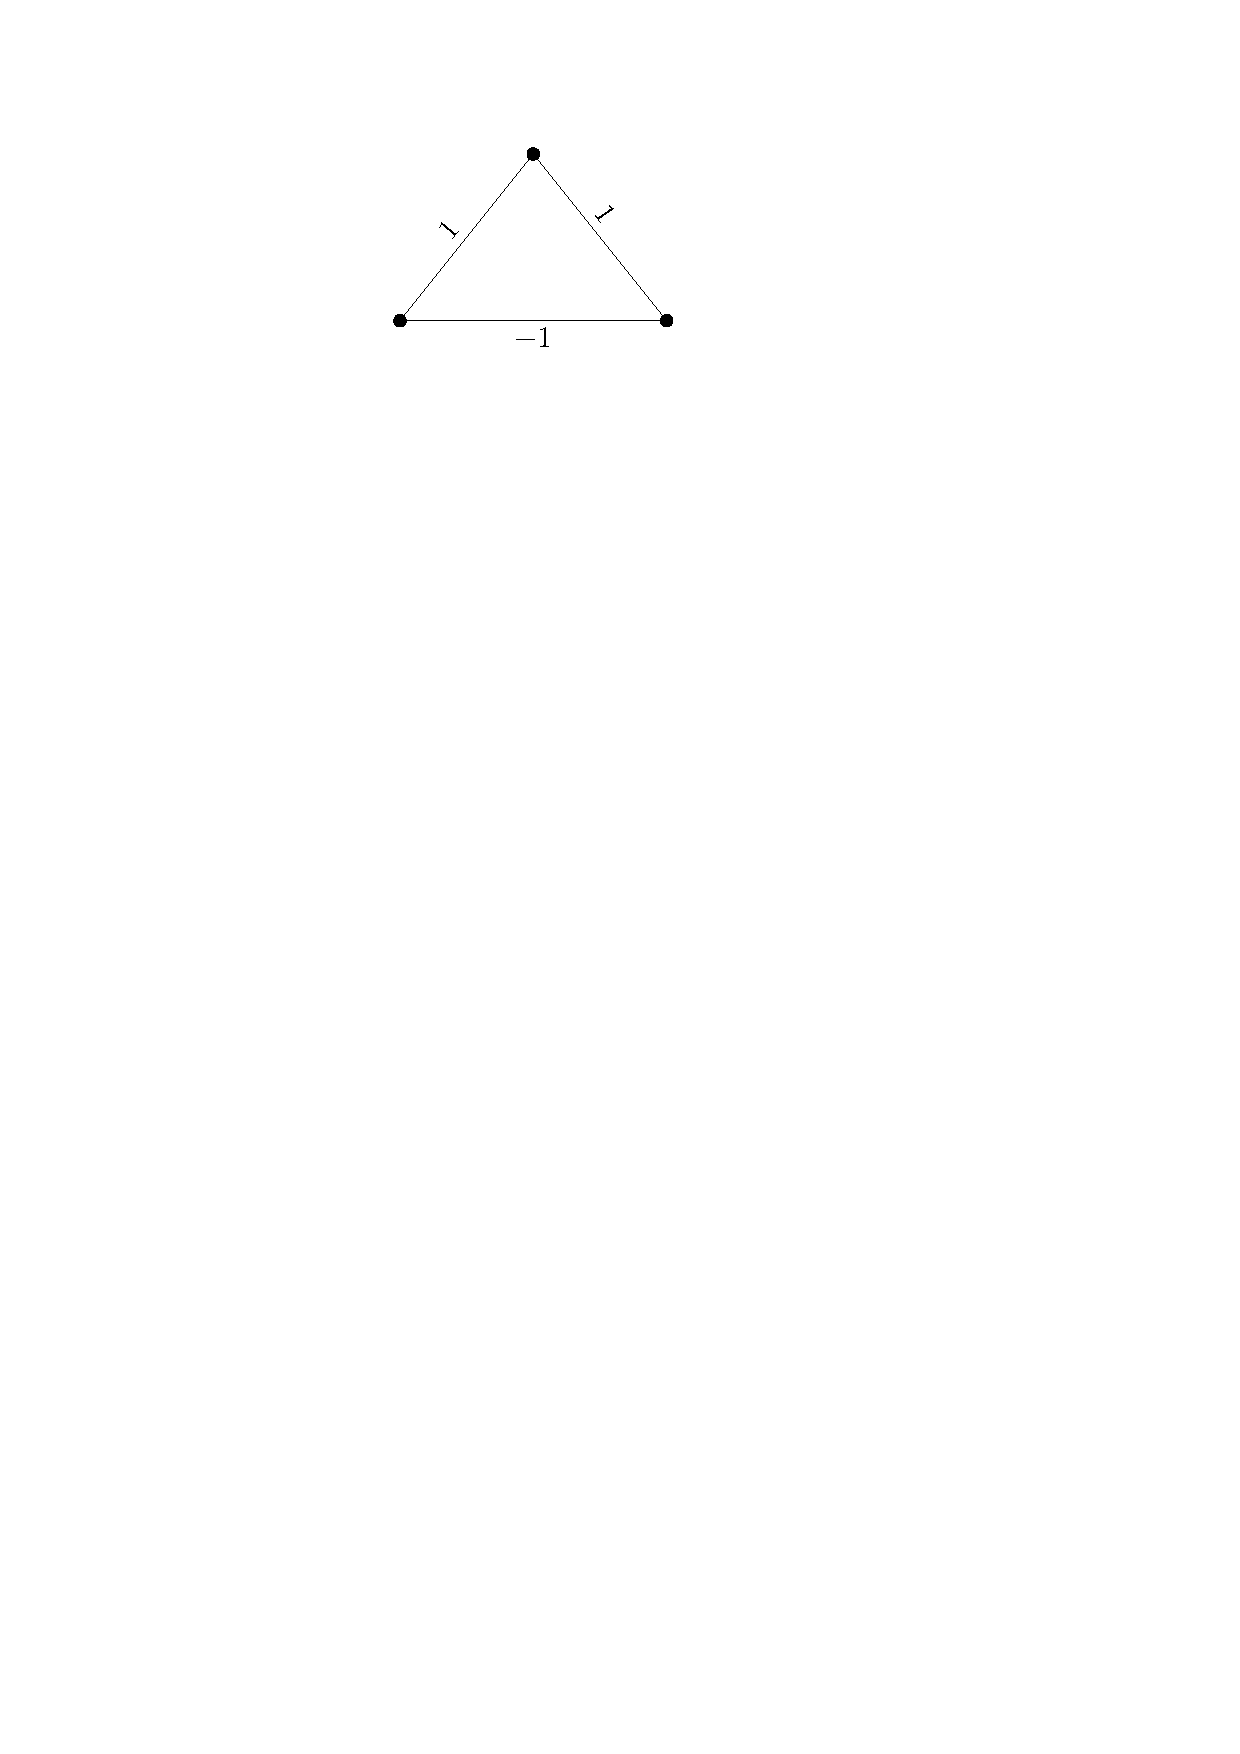
\includegraphics[width=0.25\textwidth]{figures/arbitrary-weighted-graph-score.pdf}
\end{center}
This ``graph with real edge weights'' has score $(2,0,0)$. This score is impossible for
graphs, multigraphs, and weighted graphs with non-negative edge weights.


\begin{exercise}
  State a score theorem for weighted graphs when we allow
  negative edge weights. That is, state a theorem like \emph{if we view the edge between vertex $i,j$ with weight $x_{ij}$ as unknown numbers, then we can write down equations like}
  \begin{align*}
    \sum_{j=1,2,\cdots,i-1,i+1,\cdots,n}x_{ij}=a_i,
  \end{align*}
\emph{where $a_i$ is the degree of $i$-th vertex in the score. If and only if we can find a solution for these equations, then there exists a graph with real edge weights with this score.}

\emph{To make this criteria explicit, let us use the aid of linear algebra. Say, $\mathbf{x}=(x_{12},x_{13},\cdots,x_{1n},x_{23},x_{24},\cdots,x_{n-1,n})^T$ is an ${n \choose 2}\times 1$ vector with no repeating elements. $\mathbf{\beta}=(a_1,\dots,a_n)^T$ is an $n\times 1$ vector. $\mathbf{A}$ is an $n\times {n\choose 2}$ matrix whose elements are coefficients in the equations mentioned above, so that the equation in matrix form}
\begin{align}\label{eq-matrix}
  \mathbf{Ax}=\beta
\end{align}
\emph{holds. Let $\widetilde{\mathbf{A}}$ denote the argumented matrix of $\mathbf{A}$. We know that the equation group~\eqref{eq-matrix} has a solution if and only if \textnormal{r($\mathbf{A}$)=r($\mathbf{\widetilde{A}}$)}. But we can further claim that}
\begin{lemma}\label{lem-fullrank}
  For any $n>2$, equation group~\eqref{eq-matrix} satisfies that \textnormal{r($\mathbf{A}$)=r($\mathbf{\widetilde{A}}$)}=$n$.
\end{lemma}
\begin{proof}
  The argumented matrix $\mathbf{\widetilde{A}}$ has the form\begin{align*}
    \setcounter{MaxMatrixCols}{14}
    \mathbf{\widetilde{A}}=
    \begin{matrix}
         \begin{bmatrix}
        1&1&1&\cdots&1&0&\cdots&0&0&\cdots&0&a_1\\
        1&0&0&\cdots&0&1&\cdots&1&0&\cdots&0&a_2\\
        0&1&0&\cdots&0&1&\cdots&0&1&\cdots&0&a_3\\
        \vdots&\vdots&\vdots&&\vdots&\vdots&&\vdots&\vdots&&\vdots&\vdots\\
        0&0&0&\cdots&1&0&\cdots&0&0&\cdots&1&a_n
      \end{bmatrix},
    \end{matrix}
  \end{align*}
  
  when $n>2$, we can always change it into the following form via elementary row operations:
  \begin{align*}
    \setcounter{MaxMatrixCols}{14}
    \mathbf{\widetilde{A}}=
    \begin{matrix}
      \begin{bmatrix}
        1&\;\;1&1&\cdots&\;1&\;\;0&\;\;\cdots&0&0&\cdots&0&a_1\\
        0&\;\;-1&-1&\cdots&\;-1&\;\;1&\;\;\cdots&1&0&\cdots&0&a_2-a_1\\
        0&\;\;0&-1&\cdots&\;-1&\;\;2&\;\;\cdots&1&1&\cdots&0&a_3+a_2-a_1\\
        \vdots&\;\;\vdots&\vdots&&\vdots&\;\;\vdots&&\vdots&\vdots&&\vdots&\vdots\\
        0&\;\;0&0&\cdots&\;\;0&\;\;2&\;\;\cdots&2&2&\cdots&2&\sum_{i=2}^na_i-a_1
      \end{bmatrix},
    \end{matrix}
  \end{align*}
  from which we can easily see that \textnormal{r($\mathbf{A}$)=r($\mathbf{\widetilde{A}}$)}=$n$.
\end{proof}
\emph{With this we can write the theorem formally as follows:}
  \begin{theorem}[Score Theorem for Graphs with Real Edge Weights]
     Let $(a_1,\dots,a_n) \in \R^n$. There is a  graph with real edge weights
     with this score if and only if \textnormal{r($\mathbf{A}$)=r($\mathbf{\widetilde{A}}$)}. Specially, if $n>2$, there is a graph with real edge weights with this score.
  \end{theorem}  
\end{exercise}

\begin{exercise}
Prove your theorem.
\begin{proof}
  \textbf{Sufficiency.} If \textnormal{r($\mathbf{A}$)=r($\mathbf{\widetilde{A}}$)},  equation group~\eqref{eq-matrix} has a solution in $\R^n$. Specially if $n>2$,then according to Lemma~\ref{lem-fullrank}, the same statement holds. That means, we can find a complete graph with real edge weights satisfying this score.

  \textbf{Necessity.} If there is a  graph with real edge weights with this score, we can always expand the graph to a complete graph, assigning weight of 0 to the edges that previously do not exist. Then we get a solution for the equation group~\eqref{eq-matrix}, which means \textnormal{r($\mathbf{A}$)=r($\mathbf{\widetilde{A}}$)}.
\end{proof}
\end{exercise}


\begin{exercise}
   For each student ID $(a_1,\dots,a_n)$ in your group, check whether
   this is (1) a graph score, (2) a multigraph score, (3) a weighted graph score, or
   (4) the score of a graph with real edge weights.

   Whenever the answer is {\em yes}, show the graph, when it is {\em no},
   give a short argument why.
   \begin{solution} \quad
  \begin{itemize}
    \item (5,1,7,0,2,1,9,1,0,6,2,3)
    \begin{enumerate}
      \item This is not a graph score, as there are odd number of odd degrees in the score, which violates the Handshaking lemma.
      \item This is not a multigraph score, as the Handshaking lemma still holds for multigraph, and there are odd number of odd degrees in the score, which violates the Handshaking lemma.
      \item This is a weighted graph score. See the diagram of graph in Figure~\ref{fig-sty}.
      \item This is a score of graph with real edge weights, as the answer for (3) is yes.
    \end{enumerate}
    \item (5,1,7,0,2,1,9,1,0,8,8,2)

  First, this is not a graph score. According to the graph score theorem, this is a graph score iff 406010000771 is a graph score. However, $d_10=7$ but there are only five other vertices whose degree are greater than 0. Hence, this is not a graph score.

  Second, this is a multigraph score. The graph is shown below.
  

  Since this is a multigraph score, it is also a weighted graph score and the allowing negative edge weighted graph score. These two graph are the same as the following figure shows.

  

 \item (5,1,7,0,2,1,9,1,0,7,2,4)
 	\begin{enumerate}
 		\item This is neither a graph nor a multigraph because the sum of degree is odd, which go against the Handshaking Lemma.
 		\item This is a weighted graph. The figure of graph is shown below.
 		
 	\end{enumerate}

 \item (5,1,7,0,2,1,9,1,0,5,4,0)
 	\begin{enumerate}
 		\item This is neither a graph nor a multigraph because the sum of degree is odd, which go against the Handshaking Lemma.
 		\item This is a weighted graph. The figure of graph is shown below.
 		
 	\end{enumerate}
  \end{itemize}
  \begin{figure}
        \centering
        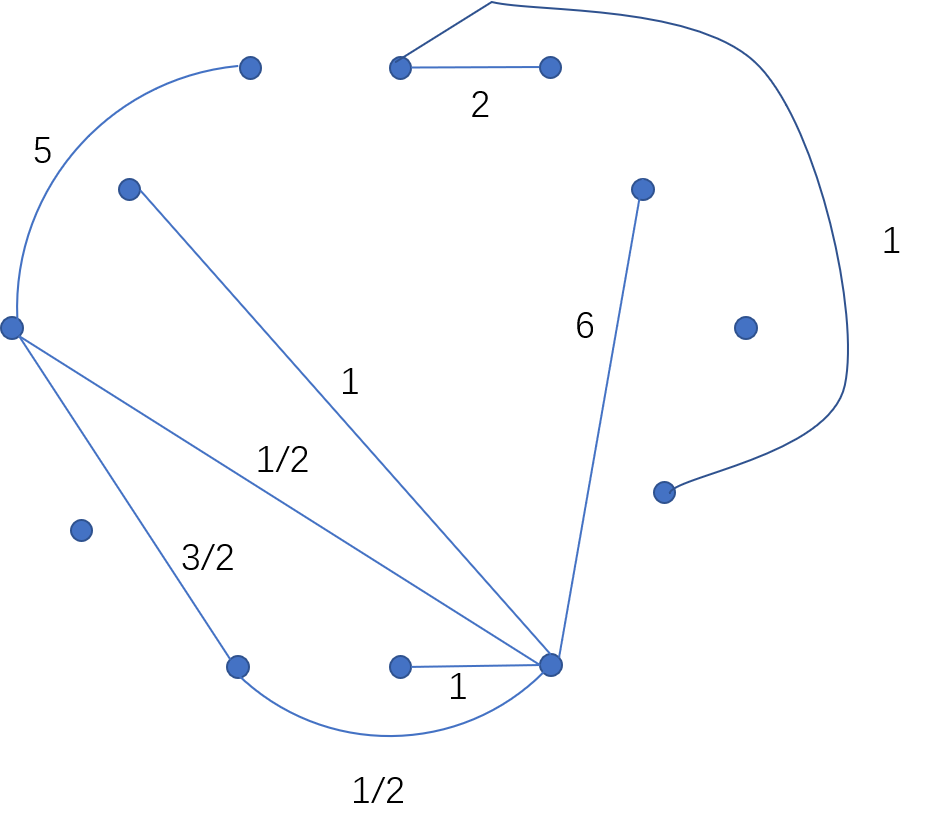
\includegraphics[width=0.5\textwidth]{figures/sty.png}\caption{weighted graph: 517021910623}\label{fig-sty}
      \end{figure}
  \begin{figure}[!htb]
      \centering
      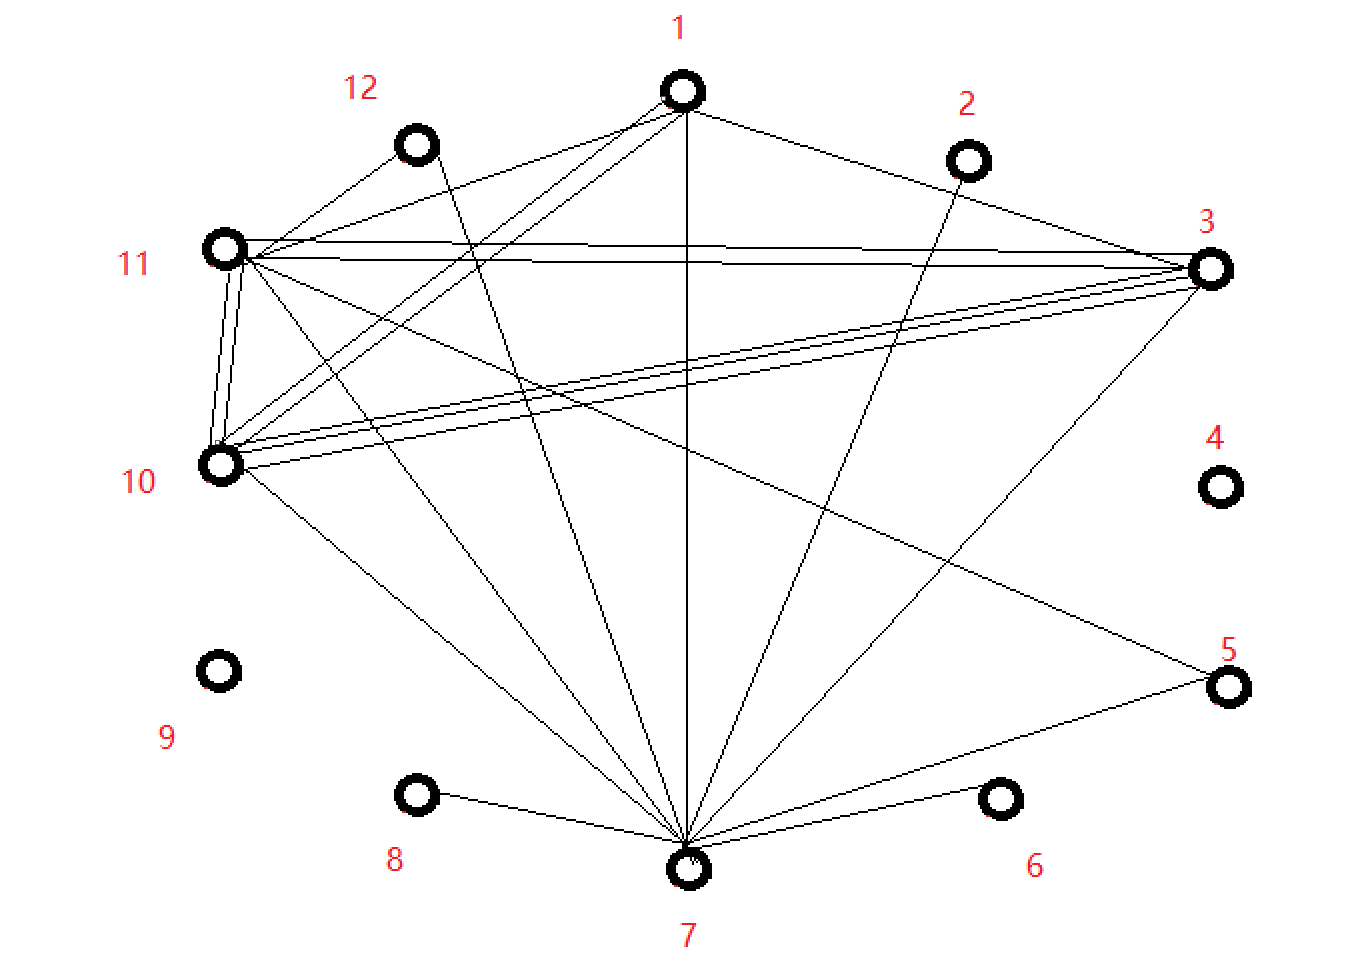
\includegraphics[width=0.5\textwidth]{4.jpg}
      \caption{Multigraph: 517021910882}
  \end{figure}
  \begin{figure}[!htb]
      \centering
      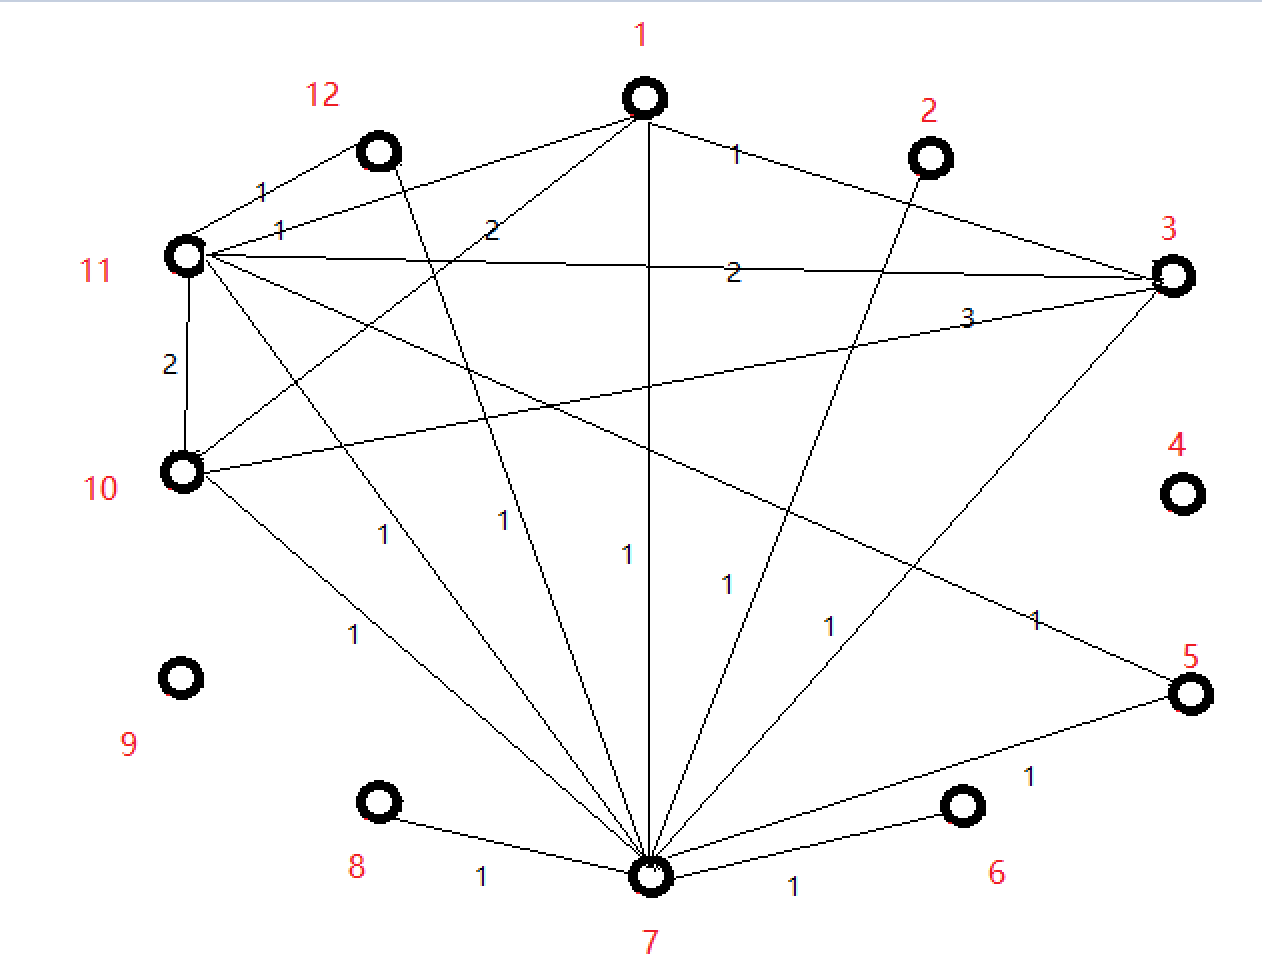
\includegraphics[width=0.5\textwidth]{5.jpg}
      \caption{Weighted graph: 517021910882}
  \end{figure}
  \begin{figure}[!htb]
     	 \centering
      	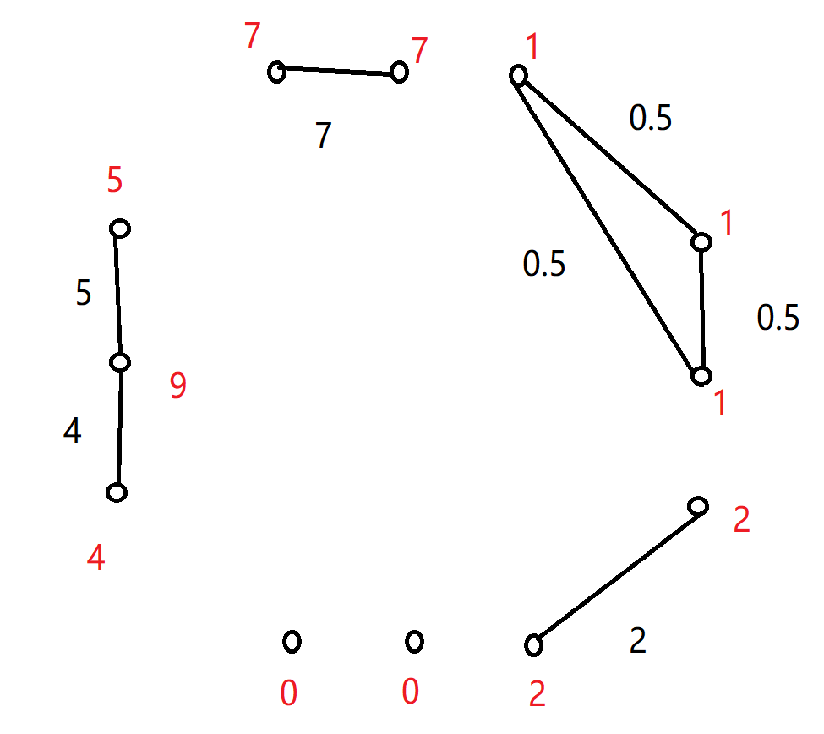
\includegraphics[width=0.5\textwidth]{p724.png}
      	\caption{Weighted graph: 517021910724}
  \end{figure}
  \begin{figure}[!htb]
      \centering
      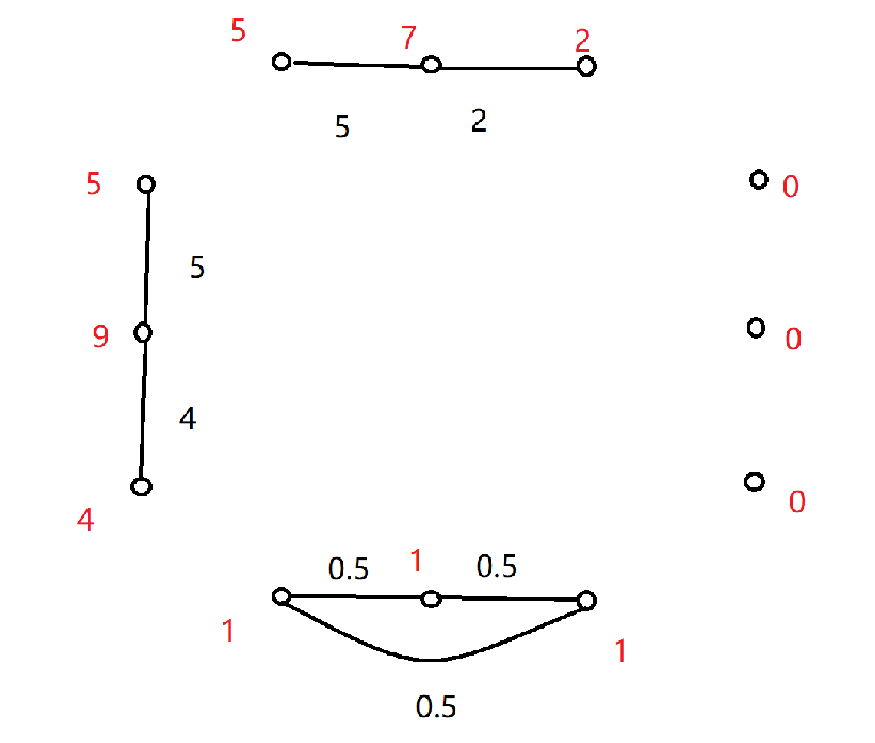
\includegraphics[width=0.5\textwidth]{p540.png}
      \caption{Weighted graph: 517021910540}
  \end{figure}
\end{solution}
\end{exercise}






\end{document}
